\subsubsection{Lift and bucket for debris}

The bucket's size allow to fit 3 cubes and 2 balls. For estimating optimal size and form was made drawing in GeoGebra.
\begin{figure}[H]
	\begin{minipage}[h]{1\linewidth}
		\center{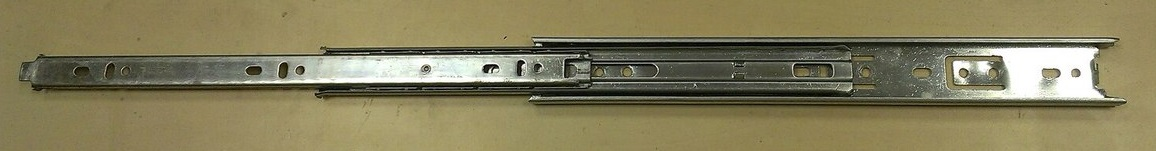
\includegraphics[scale=0.2]{daysL/Lift+bucket/images/01}}
		\caption{Drawing of the bucket}
	\end{minipage}
\end{figure}  


The lift consists of two beams. One beam is stationar and it is fixed vertically on the back part of the robot. The second beam turns by DC motor that mounted at the top of stationar beam. For estimating optimal length of beams was made drawing in GeoGebra.
\begin{figure}[H]
	\begin{minipage}[h]{1\linewidth}
		\center{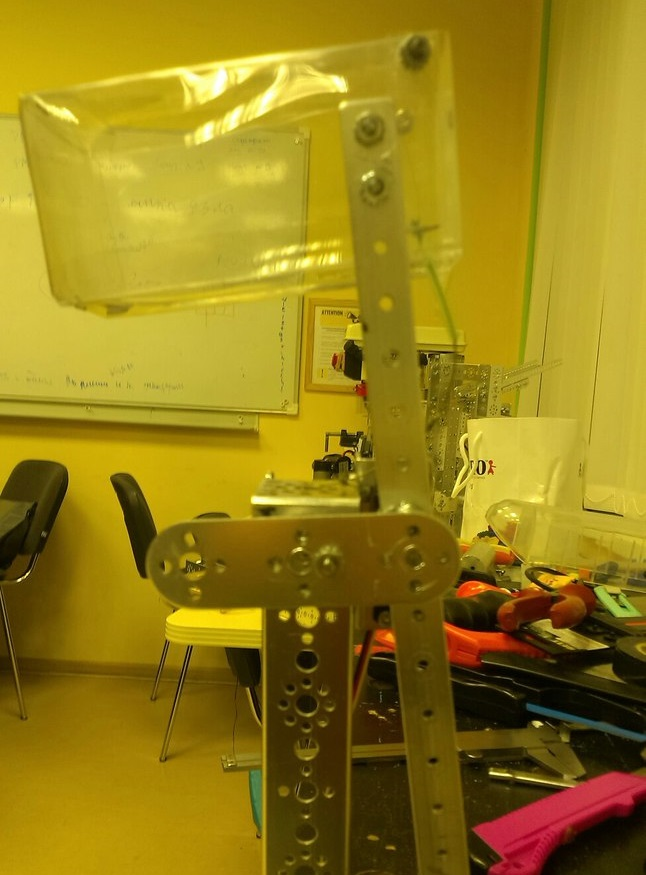
\includegraphics[scale=0.2]{daysL/Lift+bucket/images/02}}
		\caption{robot}
	\end{minipage}
\end{figure}


  	\begin{figure}[H]
  		\begin{minipage}[h]{1\linewidth}
  			\center{
\includegraphics[scale=0.2]{00.00.2015/images/02}}
  			\caption{robot}
  		\end{minipage}
  	\end{figure}
  	
   	


\fillpage
